\chapter{Results and Discussion}
\label{cha:result}
In this section we produce a synthetic computer network within Python, validating its correctness with respect to our model's assumptions in \cref{sec:Rmodelvalidation}. Once validated we apply baseline techniques introduced in \cref{cha:methodology} to test our new methods for nefarious router identification. We compared these results to previous analytical techniques, highlighting trade offs in accuracy for generally applicability, deploy-ability and run time within \cref{sec:Rnefarouterdetection}. During this analysis several interesting behaviours were encountered in edge cases, these findings are shown and further experiments conducted on hypothesised explanations for the behaviour within \cref{ssec:Rsympathicpdv} and \cref{ssec:Rmetricnormalisation}. Of particular noteworthiness is that the investigation into unexpectedly poor inferential results from router level \pdv  behaviour in \cref{ssec:Rmetricnormalisation} revealed a flaw within previous work's inferential calculation, necessitating changes to the experimental methodology. We then move to testing the impacts of optimal probe allocation techniques on our inferential accuracy in \cref{sec:Rprobingoptimality}, ...\par
\todo{Very brief outline of accuracy changes based on A/D optimality, (it went up/down by x)}
Finally we construct a simulated network using real world topological and traffic data-sets within the NS3 framework to test our new method's performance in real world networks, formulating a quantitative response to our project's overarching goal.

\section{Model Validation}
\label{sec:Rmodelvalidation}

\subsection{Queue Stabilization}
\label{ssec:Rqueuestabilization}
\todo{Need to either decompose model validation more or switch back to just "queue stability" as the section}
\begin{figure}[H]
    \centering
    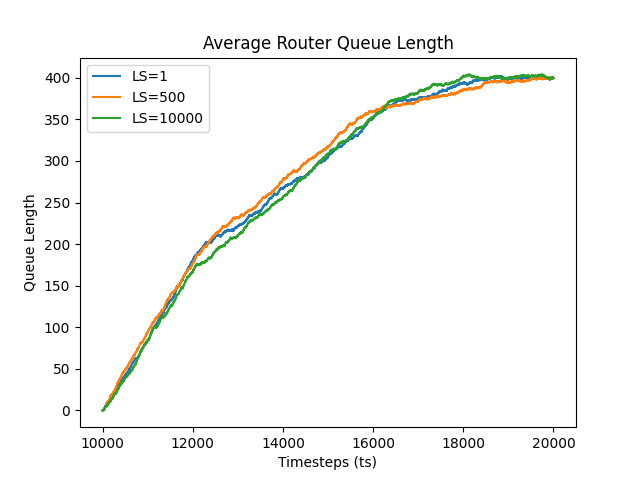
\includegraphics[width=\textwidth]{net_tom_sim/tests/steady_queue_length_tests/100000 ts 1/graphs/trimmed/average_of_1,500,10000.png}
    \caption{Average router queue buffer length over varied link-state updating intervals.}
    \label{fig:Ravgq}
\end{figure}

\begin{table}[H]
    \centering
    \begin{tabular}{||c c c||}
        \hline
        \multicolumn{3}{||c||}{Average Variance Over LS Update Intervals} \\ [0.5ex]
        \hline
        \multicolumn{1}{||c|}{Range} & $ts \leq 20,000$ & $ts > 20,000$ \\ [0.5ex]
        \hline\hline
        1       & 10,657.16 & 6.25 \\ 
        10      & 10,240.66 & 4.88 \\
        50      & 10,128.76 & 3.21 \\
        250     & 10,655.41 & 5.06 \\
        500     & 10,087.16 & 6.05 \\
        1,000   & 10,281.32 & 3.47 \\
        10,000  & 11,169.38 & 5.22 \\ [1ex] 
        \hline
    \end{tabular}
    \caption{Variance pre and post queue length stabilization point}
\end{table}
\section{Nefarious Router Detection}
\label{sec:Rnefarouterdetection}
\begin{figure}[H]
        \centering
        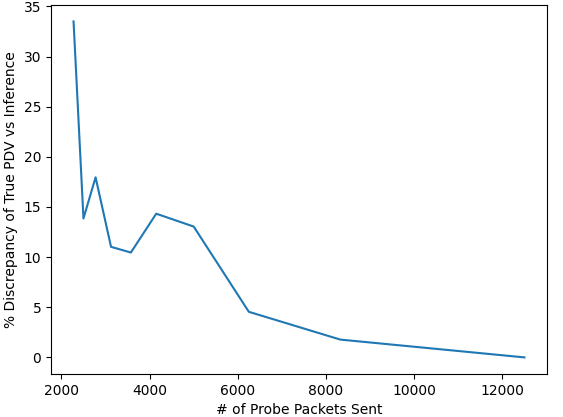
\includegraphics[width=\textwidth]{net_tom_sim/tests/manual_PDV/Probe_PDV_accuracy_plot.png}
        \caption{Accuracy of inference from true values over a range of probes sent.}
        \label{fig:Rqstabilization}
\end{figure}
\emph{Cover results in a 7 router network and resulting metric normalisation (refer to \cref{ssec:Rsympathicpdv} for 6 router) and 10 router, then for novel topologies (Peterson graph, tripartite graph)}

\subsection{Metric Normalisation}
\label{ssec:Rmetricnormalisation}
The delay distribution and by extension delay variation at a single router is intuitively a combination of the two contributors to \gls{qlen} within the system:
\begin{enumerate}
    \item The \# of packets a router receives.
    \item The \# of packets a router sends.
\end{enumerate}
Contributor \emph{2} is always a fixed rate of 1 packet per time step unless a router is nefarious in which case it will be $<1$ proportional to the router's probability of holding a packet. As the rate of sending is not impacted by contributor \emph{1} we account for variation of contributor \emph{1} between routers to increase the transparency of queuing delay due to variations by contributor \emph{2} within the network.\par
The variation in contributor \emph{1} is proportional to the degree of each node as the number of packets being received by a router each time step is the sum of packets received from each link. Initially we utilized $\sqrt{\gls{routerdeg}}$ for normalization over delay observations by taking $\forall r\in R, \frac{\sigma^2}{\sqrt{\gls{routerdeg}}}$ where $\sigma^2$ is the variance of delay measurements.
\todo{Show results for inferential accuracy RE probing a network where nefarious router has << switches than a non-nef, to demonstrates why we want to normalise for the number of links. }

\subsection{Sympathetic PDV Increases}
\label{ssec:Rsympathicpdv}


\section{Probing Optimality}
\label{sec:Rprobingoptimality}

\section{Real Network Performance}
\label{sec:Rrealnetworkperformance}

\section{Summary}
